% *********************************************************************
% © 2010–2023 Jeremy Sylvestre
%
% Permission is granted to copy, distribute and/or modify this document
% under the terms of the GNU Free Documentation License, Version 1.3 or
% any later version published by the Free Software Foundation; with no
% Invariant Sections, no Front-Cover Texts, and no Back-Cover Texts. A
% copy of the license is included in the appendix entitled “GNU Free
% Documentation License” that appears in the output document of this
% PreTeXt source code. All trademarks™ are the registered® marks of
% their respective owners.
%
% *********************************************************************

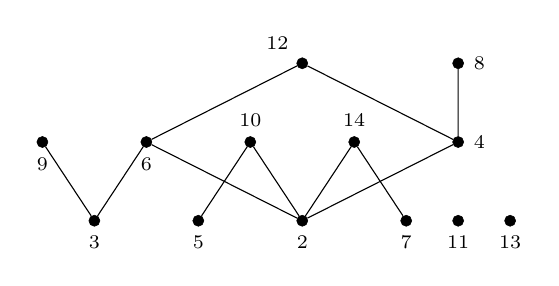
\begin{tikzpicture}[
	xscale=0.66,
	vertex/.style={ circle, draw, very thin, fill, inner sep=0pt, minimum size=4pt },
	vertexg/.style={ black!40!white, circle, draw, very thin, fill, inner sep=0pt, minimum size=4pt },
	vertexo/.style={ circle, draw, very thin, inner sep=0pt, minimum size=4pt }
]

\node at (4,0) (two) [vertex,label=below:$\scriptstyle 2$] {};
\node at (0,0) (three) [vertex,label=below:$\scriptstyle 3$] {};
\node at (2,0) (five) [vertex,label=below:$\scriptstyle 5$] {};
\node at (6,0) (seven) [vertex,label=below:$\scriptstyle 7$] {};
\node at (7,0) (eleven) [vertex,label=below:$\scriptstyle 11$] {};
\node at (8,0) (thirteen) [vertex,label=below:$\scriptstyle 13$] {};

\node at (7,1) (four) [vertex,label=right:$\scriptstyle 4$] {};
\foreach \p in {two} \draw (\p) to (four);
\node at (1,1) (six) [vertex,label=below:$\scriptstyle 6$] {};
\foreach \p in {two,three} \draw (\p) to (six);
\node at (-1,1) (nine) [vertex,label=below:$\scriptstyle 9$] {};
\foreach \p in {three} \draw (\p) to (nine);
\node at (3,1) (ten) [vertex,label=above:$\scriptstyle 10$] {};
\foreach \p in {two,five} \draw (\p) to (ten);
\node at (5,1) (fourteen) [vertex,label=above:$\scriptstyle 14$] {};
\foreach \p in {two,seven} \draw (\p) to (fourteen);
\node at (7,2) (eight) [vertex,label=right:$\scriptstyle 8$] {};
\foreach \p in {four} \draw (\p) to (eight);
\node at (4,2) (twelve) [vertex,label=above left:$\scriptstyle 12$] {};
\foreach \p in {four,six} \draw (\p) to (twelve);

\end{tikzpicture}
